\documentclass[conference]{IEEEtran}
\IEEEoverridecommandlockouts
\usepackage{cite}
\usepackage{amsmath,amssymb,amsfonts}
\usepackage{algorithmic}
\usepackage{graphicx}
\usepackage{textcomp}
\usepackage{xcolor}
\usepackage{tikz}
\usetikzlibrary{patterns,decorations.pathmorphing}
\def\BibTeX{{\rm B\kern-.05em{\sc i\kern-.025em b}\kern-.08em
    T\kern-.1667em\lower.7ex\hbox{E}\kern-.125emX}}
\begin{document}

\title{Inverse Finite Element Method for Beam Analysis}



\author{\IEEEauthorblockN{Antoine Grosse}
\IEEEauthorblockA{\textit{Institutt for marin teknikk (IMT)} \\
\textit{NTNU}\\
Trondheim, Norway \\
antoine.grosse@ntnu.no}
\and
\IEEEauthorblockN{Colin Sanguinet}
\IEEEauthorblockA{\textit{Institutt for marin teknikk (IMT)} \\
\textit{NTNU}\\
Trondheim, Norway \\
colin.sanguinet@ntnu.no}}

\maketitle

\begin{abstract}
This report gives an overview of the Inverse Finite Element Method (iFEM) for beam analysis, including its theoretical foundations, implementation details, and potential applications. The iFEM approach allows for the reconstruction of structural displacements and strains from measured data, providing a powerful tool for structural health monitoring and damage detection in beam-like structures.
\end{abstract}

\begin{IEEEkeywords}
iFEM, Inverse Finite Element Method, Beam Analysis
\end{IEEEkeywords}

\section{Introduction}
The main objective of this report is to give a general overview of the possibilities given by the Inverse Finite Element Method (iFEM) for beam structures. The iFEM is a computational technique that allows for the reconstruction of structural displacements and strains from measured data, providing a powerful tool for structural health monitoring, damage detection and model testing in experimental environment.
The aim is also to identify the limits of such a tool in regards of mesh, noise and model error sensitivities.
\section{Methodology}
\subsection{Geometry of the problem}
\begin{figure}[htbp]
\centering
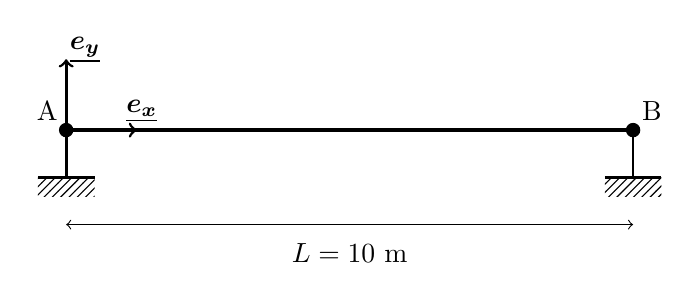
\begin{tikzpicture}[scale=1.2]
  % Beam
  \draw[line width=1.5pt] (0,0) -- (6,0);
  
  % Left support 
  \draw[fill=black] (0,0) circle (2pt);
  \node at (-0.2, 0.2) {A};
  \draw[line width=1pt] (0,0) -- (0,-0.5);
  \fill[pattern=north east lines] (-0.3,-0.5) rectangle (0.3,-0.7);
  \draw[line width=1pt] (-0.3,-0.5) -- (0.3,-0.5);
  
  % Right support 
  \draw[fill=black] (6,0) circle (2pt);
  \node at (6.2,0.2) {B};
  \draw[line width=1pt] (6,0) -- (6,-0.5);
  \fill[pattern=north east lines] (5.7,-0.5) rectangle (6.3,-0.7);
  \draw[line width=1pt] (5.7,-0.5) -- (6.3,-0.5);
  
  % Dimensions
  \draw[<->] (0,-1.0) -- (6,-1.0);
  \node at (3,-1.3) {$L = 10$ m};
  
  % Load (optional)
  \draw[->,line width=1pt] (0,0) -- (0,0.75);
  \draw[->,line width=1pt] (0,0) -- (0.75,0);
  \node at (0.8,0.2) {$\underline{\boldsymbol{e_x}}$};
  \node at (0.2,0.85) {$\underline{\boldsymbol{e_y}}$};
  
\end{tikzpicture}
\caption{Simply supported beam configuration}
\label{fig:beam_geometry}
\end{figure}
The work carried out on all of this report was done on a simply supported beam clamped at both ends as shown in figure \ref{fig:beam_geometry}. The length of the beam is 10 m. Different load scenarii were tested such as point load and distributed load.
This means that the following boundary conditions were applied:
\begin{itemize}
    \item Point A: $u_x = u_y = 0$, $\theta_z = 0$
    \item Point B: $u_x = u_y = 0$, $\theta_z = 0$
\end{itemize}
Where $u_x$ and $u_y$ are the displacements in the x and y directions respectively.

\subsection{Element type}

Euler Beam elements were used for the discretization of the beam structure. These elements are suitable for slender beams where shear deformation is negligible.
Using 4 Gauss Point for the shape functions integration. The residual is following the principle of virtual work.
\begin{equation}
R = \int_{L} \delta \epsilon^T \sigma dL - \int_{L} \delta u^T b dL - \sum_{i=1}^{nLoad} \delta u_i^T Q_i
\end{equation}
\textcolor{red}{More info on the specificity of the beam}


\subsection{Material properties}
Unit mass, unit loacal inertia, Young's modulus of 210e9 Pa and a cross section of 0.01 m2 were used for the beam.
Make a table of the properties used.
\begin{table}[htbp]
\caption{Material properties}
\begin{center}
\begin{tabular}{|c|c|c|}
\hline
\textbf{Property} & \textbf{\textit{Value}}& \textbf{\textit{Units}} \\
\hline
Axial Stiffness,  $EA$ & $10^6$ & m/N\\
Bending Stiffness along $\underline{\boldsymbol{e_y}}$, $EI_1$& $10^5$ & N.$\text{m}^2$ \\
Bending Stiffness along $\underline{\boldsymbol{e_z}}$, $EI_2$& $10^5$ & N.$\text{m}^2$ \\
Torsional Stiffness, $GJ$& $10^6$ & N.$\text{m}^2$\\
Linear mass along main axis, $\mu_1$& $1.0$ & kg/m \\
Mass moment of inertia around main axis, $\iota_1$& $1.0$ & kg.$\text{m}^3$ \\
\hline
\end{tabular}
\label{tab1}
\end{center}
\end{table}

\subsection{Load Scenarii}

To investigate the limits of the iFEM approach for beam analysis, several load scenarii were considered. These scenarii include both static and dynamic loading conditions to assess the method's performance under different circumstances.  
\subsubsection{Nodal load (Static/Dynamic/Quasi-static)}
A local load is applied at the mid span to the i-th node of the beam as shown in figure \ref{fig:Nodal_Load}.
Depending on the studied case $\underline{\boldsymbol{F}}$ can take different forms such as a step load or a sinusoidal load.

\begin{figure}[h!tbp]
\centering
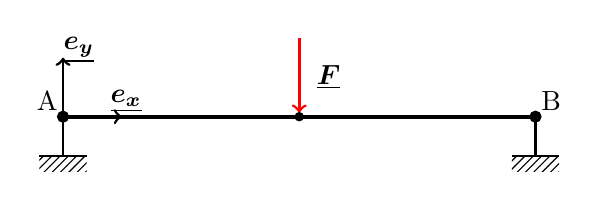
\begin{tikzpicture}[scale=1]
  % Beam
  \draw[line width=1.5pt] (0,0) -- (6,0);
  
  % Left support 
  \draw[fill=black] (0,0) circle (2pt);
  \node at (-0.2, 0.2) {A};
  \draw[line width=1pt] (0,0) -- (0,-0.5);
  \fill[pattern=north east lines] (-0.3,-0.5) rectangle (0.3,-0.7);
  \draw[line width=1pt] (-0.3,-0.5) -- (0.3,-0.5);
  
  % Right support 
  \draw[fill=black] (6,0) circle (2pt);
  \node at (6.2,0.2) {B};
  \draw[line width=1pt] (6,0) -- (6,-0.5);
  \fill[pattern=north east lines] (5.7,-0.5) rectangle (6.3,-0.7);
  \draw[line width=1pt] (5.7,-0.5) -- (6.3,-0.5);

  % Nodal Load
  \draw[<-,line width=1pt,color=red] (3,0.05) -- (3,1);
  \node[anchor = west] at (3.1,0.5) {$\underline{\boldsymbol{F}}$};
  \draw[fill=black] (3,0) circle (1.5pt);
  
  % Load (optional)
  \draw[->,line width=1pt] (0,0) -- (0,0.75);
  \draw[->,line width=1pt] (0,0) -- (0.75,0);
  \node at (0.8,0.2) {$\underline{\boldsymbol{e_x}}$};
  \node at (0.2,0.85) {$\underline{\boldsymbol{e_y}}$};
  
\end{tikzpicture}
\caption{Local nodal load configuration}
\label{fig:Nodal_Load}
\end{figure}

\subsubsection{Distributed load: Uniform (Dynamic)}
Distributed loads are quite common in structural applications. A uniform distributed load is applied along the entire length of the beam as shown in figure \ref{fig:Uniform_Load}. The load intensity can vary with time, allowing for dynamic analysis of the beam under such loading conditions.
\begin{figure}[h!tbp]
\centering
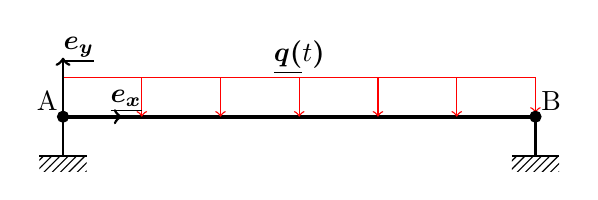
\begin{tikzpicture}[scale=1]
  % Beam
  \draw[line width=1.5pt] (0,0) -- (6,0);

  % Uniform Load
  \draw[-,line width=0.5pt,color=red] (0,0.5) -- (6,0.5);
  \draw[<-,line width=0.5pt,color=red] (3,0) -- (3,0.5);
  \draw[<-,line width=0.5pt,color=red] (1,0) -- (1,0.5);
  \draw[<-,line width=0.5pt,color=red] (2,0) -- (2,0.5);
  \draw[<-,line width=0.5pt,color=red] (4,0) -- (4,0.5);
  \draw[<-,line width=0.5pt,color=red] (5,0) -- (5,0.5);
  \draw[<-,line width=0.5pt,color=red] (6,0.05) -- (6,0.5);
  \node[anchor = center] at (3,0.75) {$\underline{\boldsymbol{q(}}t \boldsymbol{)}$};
  
  % Left support 
  \draw[fill=black] (0,0) circle (2pt);
  \node at (-0.2, 0.2) {A};
  \draw[line width=1pt] (0,0) -- (0,-0.5);
  \fill[pattern=north east lines] (-0.3,-0.5) rectangle (0.3,-0.7);
  \draw[line width=1pt] (-0.3,-0.5) -- (0.3,-0.5);
  
  % Right support 
  \draw[fill=black] (6,0) circle (2pt);
  \node at (6.2,0.2) {B};
  \draw[line width=1pt] (6,0) -- (6,-0.5);
  \fill[pattern=north east lines] (5.7,-0.5) rectangle (6.3,-0.7);
  \draw[line width=1pt] (5.7,-0.5) -- (6.3,-0.5);

  
  
  
  % Load (optional)
  \draw[->,line width=1pt] (0,0) -- (0,0.75);
  \draw[->,line width=1pt] (0,0) -- (0.75,0);
  \node at (0.8,0.2) {$\underline{\boldsymbol{e_x}}$};
  \node at (0.2,0.85) {$\underline{\boldsymbol{e_y}}$};
  
\end{tikzpicture}
\caption{Uniform distributed load configuration}
\label{fig:Uniform_Load}
\end{figure}

\subsubsection{Distributed load: 2nd mode shape (Dynamic)}

To get near free vibration condition, a sinusoidally distributed load is applied along the entire length of the beam as shown in figure \ref{fig:2nd_Mode_Load}. The load intensity varies with both time and position along the beam, following the second mode shape of vibration.

\begin{figure}[h!tbp]
\centering
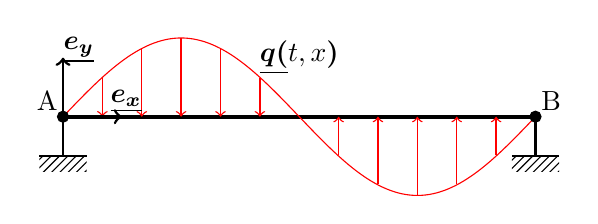
\begin{tikzpicture}[scale=1]
  % Beam
  \draw[line width=1.5pt] (0,0) -- (6,0);
  
  % Uniform Load
  \draw[color=red] (0,0) sin (1.5,1) cos (3,0) sin (4.5,-1) cos (6,0);
  \draw[<-,line width=0.5pt,color=red] (1.5,0) -- (1.5,1);
  \draw[<-,line width=0.5pt,color=red] (1,0) -- (1,0.86);
  \draw[<-,line width=0.5pt,color=red] (2,0) -- (2,0.86);
  \draw[<-,line width=0.5pt,color=red] (4,0) -- (4,-0.86);
  \draw[<-,line width=0.5pt,color=red] (5,0) -- (5,-0.86);
  \draw[<-,line width=0.5pt,color=red] (4.5,0) -- (4.5,-1);
  \draw[<-,line width=0.5pt,color=red] (5.5,0) -- (5.5,-0.49);
  \draw[<-,line width=0.5pt,color=red] (3.5,0) -- (3.5,-0.49);
  \draw[<-,line width=0.5pt,color=red] (2.5,0) -- (2.5,0.49);
  \draw[<-,line width=0.5pt,color=red] (0.5,0) -- (0.5,0.49);
  \node[anchor = center] at (3,0.75) {$\underline{\boldsymbol{q(}}t, x \boldsymbol{)}$};

  % Left support 
  \draw[fill=black] (0,0) circle (2pt);
  \node at (-0.2, 0.2) {A};
  \draw[line width=1pt] (0,0) -- (0,-0.5);
  \fill[pattern=north east lines] (-0.3,-0.5) rectangle (0.3,-0.7);
  \draw[line width=1pt] (-0.3,-0.5) -- (0.3,-0.5);
  
  % Right support 
  \draw[fill=black] (6,0) circle (2pt);
  \node at (6.2,0.2) {B};
  \draw[line width=1pt] (6,0) -- (6,-0.5);
  \fill[pattern=north east lines] (5.7,-0.5) rectangle (6.3,-0.7);
  \draw[line width=1pt] (5.7,-0.5) -- (6.3,-0.5);

  
  
  
  % Load (optional)
  \draw[->,line width=1pt] (0,0) -- (0,0.75);
  \draw[->,line width=1pt] (0,0) -- (0.75,0);
  \node at (0.8,0.2) {$\underline{\boldsymbol{e_x}}$};
  \node at (0.2,0.85) {$\underline{\boldsymbol{e_y}}$};
  
\end{tikzpicture}
\caption{Sinusoidally distributed load configuration}
\label{fig:2nd_Mode_Load}
\end{figure}

\subsection{Inverse simulation}

The typical costs used were... We pretend that all nodes have a known cost and all.

\section{Results}
\subsection{Inverse crime}
Everything is perfect, no noise, same mesh, same model.
\subsection{Mesh sensibility}
Local node disappears, uniform mesh coarsening, knowledge of the displacement of only some nodes
\subsection{Noise sensibility}
\subsection{Model knowledge}

Inexact knowledge of the material properties (E, I, $\rho$, A), from XU to XUA.

\subsection{Time discretization sensibility}
Shannon and potential difference in discretization between interpolated measurments and inverse method


\section{Conclusion}

 





\end{document}